\chapter{Anforderungsdefinition und Modellierung}
\label{cha:Anforderungsdefinition und Modellierung}

In diesem Kapitel definieren wir die funktionalen Anforderungen des Softwareprojektes für die ausgesuchten Strategiespiele, den Zufallsagenten, den Heuristik Agenten, den TD-Q-Agenten und die Agententests. Anschließend werden wir die funktionalen Anforderungen und die Zusammenhänge in einem Klassendiagramm veranschaulichen. \\

Bisher war geplant, für Reversi genau wie für Tic Tac Toe, das TD-Q-Lernen zu implementieren. Anhand der Tests der unterschiedlich großen Tic Tac Toe Spielfelder, werden wir ableiten können, dass bereits eine kleine Veränderung der Dimension des Spielfelds eine enorme Rechenzeitverlängerung der Lernphasen bedeutet. Wir können daraus schlussfolgern, dass das TD-Q-Lernen, mit tabellarischer Q-Funktionsrepräsentation, für Reversi nicht geeignet ist. Diese Aussage wird in der Auswertung bewiesen, deshalb werden wir den TD-Q-Agenten für Reversi nicht mehr implementieren. \\

\section{Funktionale Anforderungen}
\label{sec:Funktionale Anforderungen}
Im nachfolgenden Abschnitt definieren wir die funktionalen Anforderungen der Software. Wir bestimmten, welche Funktionalitäten die Strategiespiele und die Agenten mindestens haben müssen und wie die Agenten getestet werden sollen. Wir definieren die Funktionalitäten, um den Funktionsbereich der Software einzugrenzen und einen Überblick zu verschaffen.
\newpage

\subsection{Tic Tac Toe Spielumgebung}
\myparagraph{class TicTacToe:}
Die Spielumgebung soll die in Abschnitt \ref{sec:Das Strategiespiel Tic Tac Toe} definierten Tic Tac Toe Spielregeln implementieren. Die Tic Tac Toe Spielumgebung repräsentiert eine Testumgebung für die Agenten. Der Zufallsagent wird in dieser Umgebung gegen den TicTacToe-Heuristik Agenten antreten. Der TD-Q-Agent soll zuerst diese Umgebung erkunden und lernen, sich in der Umgebung zurecht zu finden, d.h. der TD-Q-Agent soll eine TicTacToe-Siegesstrategie entwickeln. 

\myparagraph{makeMove(position):}
Die Funktion soll Koordinaten erhalten. Die Koordinaten definiert exakt, auf welches Spielfeld eine Spielfigur gesetzt werden soll. Die Funktion soll diesen Spielzug, sollte dieser Regelkonform sein, ausführen.

\myparagraph{undoMove():}
Die Funktion soll den letzten durchgeführten Spielzug revidieren.

\myparagraph{getPossibleMoves(): return list}
Die Funktion soll eine Liste von Koordinaten liefern. In dieser Liste sind nur mögliche und regelkonforme Spielzüge (Koordinaten) enthalten.

\myparagraph{getPlayerToMove(): return str}
Die Funktion soll einen String zurückgeben. Dieser String repräsentiert den Spieler der aktuell einen Spielzug ausführen soll. Der String ''X'' ist die Repräsentation des Kreuzspielers. Der String ''O'' ist die äquivalente Repräsentation des Kreisspielers.

\myparagraph{isTerminal: return bool}
Die Funktion soll True zurück liefern, wenn der aktuelle Zustand der Umgebung ein Endzustand (Terminalzustand) ist, andernfalls liefert die Funktion ein False.

\myparagraph{getReward: return float}
Die Funktion soll eine nummerische Belohnung liefern. Die Belohnung soll abhängig sein vom aktuellen Spielzustand.
\newpage

\subsection{Reversi Spielumgebung}
\myparagraph{class Reversi:}
Die Spielumgebung soll die in Abschnitt \ref{sec:Das Strategiespiel Reversi} definierten Reversi Spielregeln implementieren. Die Reversi Spielumgebung repräsentiert eine Testumgebung für die Agenten. Der Zufallsagent wird in dieser Umgebung gegen den Reversi-Heuristik Agenten antreten. Der TD-Q-Agent soll zuerst diese Umgebung erkunden und lernen, sich in der Umgebung zurecht zu finden, d.h. der TD-Q-Agent soll eine Reversi-Siegesstrategie entwickeln. 

\myparagraph{makeMove(position):}
Die Funktion soll Koordinaten erhalten. Die Koordinaten definiert exakt, auf welches Spielfeld eine Spielfigur gesetzt werden soll. Die Funktion soll diesen Spielzug, sollte dieser Regelkonform sein, ausführen.

\myparagraph{undoMove():}
Die Funktion soll den letzten durchgeführten Spielzug revidieren.

\myparagraph{getPossibleMoves(): return list}
Die Funktion soll eine Liste von Koordinaten liefern. In dieser Liste sind nur mögliche und regelkonforme Spielzüge (Koordinaten) enthalten.

\myparagraph{getPlayerToMove(): return str}
Die Funktion soll einen String zurückgeben. Dieser String repräsentiert den Spieler der aktuell einen Spielzug ausführen soll. Der String ''B'' ist die Repräsentation des schwarzen (black) Spielers. Der String ''W'' ist die äquivalente Repräsentation des weißen (white) Spielers.

\myparagraph{isTerminal: return bool}
Die Funktion soll True zurück liefern, wenn der aktuelle Zustand der Umgebung ein Endzustand (Terminalzustand) ist, andernfalls liefert die Funktion ein False.

\myparagraph{getReward: return float}
Die Funktion soll eine nummerische Belohnung liefern. Die Belohnung soll abhängig sein vom aktuellen Spielzustand.
\newpage

\subsection{Agent des Zufalls}
\myparagraph{class RandomAgent:}
Der Agent des Zufalls soll den Spieler symbolisieren, der keine Strategie hat und nicht lernt. Er soll seine Entscheidungen vollkommen zufällig treffen. In Kapitel \ref{cha:Validierung} Validierung werden wir diesen Agenten, als Gegenspieler für die Heuristik Agenten und die lernenden TD-Q-Agenten einsetzen. \\

\myparagraph{suggestRandomTicTacToeAction(ticTacToeState): return tuple}
Diese Funktion soll eine Tic Tac Toe Spielsituation übergeben bekommen, d.h. eine Instanz der TicTacToe-Klasse. Die Funktion soll eine zufällige, aber zulässige Aktion zurückgeben.

\myparagraph{suggestRandomReversiAction(reversiState): return tuple}
Diese Funktion soll eine Reversi Spielsituation übergeben bekommen, d.h. eine Instanz der Reversi-Klasse. Die Funktion soll eine zufällige, aber zulässige Aktion zurückgeben.

\subsection{Tic Tac Toe Heuristik Agent}
\myparagraph{class TicTacToeHeuristicSearchAgent:}
Der Agent soll die in Abschnitt \ref{subsec:Tic Tac Toe Heuristik} erstellte Tic Tac Toe Heuristik und eine 2-Spielzüge vorausschauende Alpha-Beta Suche verwenden. Dieser Agent soll einen fortgeschrittenen Spielgegner repräsentiert, d.h. wir müssen mittels Testspielen gegen den Zufallsagenten zeigen, dass der Tic Tac Toe Heuristik Agent verhältnismäßig oft gewinnt. Dieser Agent soll in Tic Tac Toe Testspielen gegen den TD-Q-Agenten antreten. Die Ergebnisse sollen dabei helfen, die Leistungsfähigkeit und Grenzen des TD-Q-Lernens, hinsichtlich des Lernens von Tic Tac Toe, zu beurteilen. 

\myparagraph{suggestAction(ticTacToeState): return tuple}
Diese Funktion soll eine Tic Tac Toe Spielsituation (eine Instanz der TicTacToe-Klasse) übergeben bekommen. Die Funktion soll, abhängig von der erhaltenen Spielsituation, eine Aktion vorschlagen. Die Aktion soll mittels der Tic Tac Toe Heuristik und einer 2-Zug Vorausschau und Alpha-Beta-Suche ermittelt werden.
\newpage

\subsection{Reversi Heuristik Agent}
\myparagraph{class ReversiHeuristicSearchAgent:}
Der Agent soll die in Abschnitt \ref{subsec:Reversi Heuristik} erstellte Reversi Heuristik und eine 2-Spielzüge vorausschauende Alpha-Beta Suche verwenden. Dieser Agent soll einen fortgeschrittenen Spielgegner repräsentieren, d.h. wir müssen mittels Testspielen gegen den Zufallsagenten zeigen, dass der Reversi-Heuristik Agent verhältnismäßig oft gewinnt.

\myparagraph{suggestAction(reversiState): return tuple}
Diese Funktion soll eine Reversi Spielsituation (eine Instanz der Reversi-Klasse) übergeben bekommen. Die Funktion soll, abhängig von der erhaltenen Spielsituation, eine Aktion vorschlagen. Die Aktion soll mittels der Reversi Heuristik und einer 2-Zug Vorausschau und Alpha-Beta-Suche ermittelt werden.

\subsection{Tic Tac Toe TD-Q-Agent}
\myparagraph{class TicTacToeTDQLearningAgent:}
Der Agent soll mittels des in Abschnitt \ref{subsec:Q-Lernen} behandelten TD-Q-Lernens, eine Siegesstrategie für das Strategiespiel 9 und 16 Spielfelder Tic Tac Toe entwickeln. 

\myparagraph{learnTicTacToeInXGames(amountOfGames):}
Die Funktion soll den Lernmodus des Agenten realisieren. Der Eingabeparameter legt die Anzahl der Trainingsspiele fest. Die Lernerfahrungen während dieser Trainingsspiele, sollen in einer SQLite Datenbank gespeichert werden. Für jede der 6 Trainingsphase (3 für 9 und 3 für 16 Spielfelder Tic Tac Toe) wird eine eigene Datenbank erstellt.

\myparagraph{suggestAction(ticTacToeState): return tuple}
Die Funktion soll eine Tic Tac Toe Spielsituation übergeben bekommen. Ausgehend von der Eingangsspielsituation, ist nur eine bestimmte Anzahl von Aktionen möglich. Abhängig von seinen Erfahrungen (SQL-Datenbank - Q-Funktion) und dem gegebenen Spielzustand, soll der Agent die mögliche Aktion mit dem höchsten gelernten Q-Wert zurückgeben.
\newpage

\subsection{Agententests in 9 Spielfelder Tic Tac Toe}
\myparagraph{class TestAgentsIn9FieldTicTacToe100Testgames:}
Wir testen in dieser Testklasse 3 gelernte TD-Q-Strategien (100, 1.000 und 10.000 Trainingsspiele) für das 9 Spielfelder Tic Tac Toe. Die Funktionen unterscheiden zwischen beginnendem TD-Q-Agent oder beginnendem Gegenspieler (Zufallsagent oder Heuristik Agent). In jeder Funktion der Testklasse werden genau 100 Testspiele durchgeführt.

\subsection{Agententests in 16 Spielfelder Tic Tac Toe}
\myparagraph{class TestAgentsIn16FieldTicTacToe100Testgames:}
Wir testen in dieser Testklasse 3 gelernte TD-Q-Strategien (100, 1.000 und 10.000 Trainingsspiele) für das 16 Spielfelder Tic Tac Toe. Die Funktionen unterscheiden zwischen beginnendem TD-Q-Agent oder beginnendem Gegenspieler (Zufallsagent oder Heuristik Agent). In jeder Funktion der Testklasse werden genau 100 Testspiele durchgeführt.

\myparagraph{Beispielfunktion $\rightarrow$  testTDQ100AgainstFirstMoveRandomAgent():}
In dieser Funktion spielen der TD-Q-Agent (100 Trainingsspiele Strategie) und der Zufallsagent gegeneinander. Der Zufallsagent beginnt das Spiel.


\section{Modellierung}
Die Zusammenhänge der Anforderungen sind im nachfolgenden Klassendiagramm (siehe Abbildung \ref{fig:klassendiagramm}) dargestellt. \\

In diesem Klassendiagramm sind die im Abschnitt \ref{sec:Funktionale Anforderungen} beschriebenen Funktionen vollständig  wiedergegeben. \\

\begin{figure}[!htbp]
  \centering
  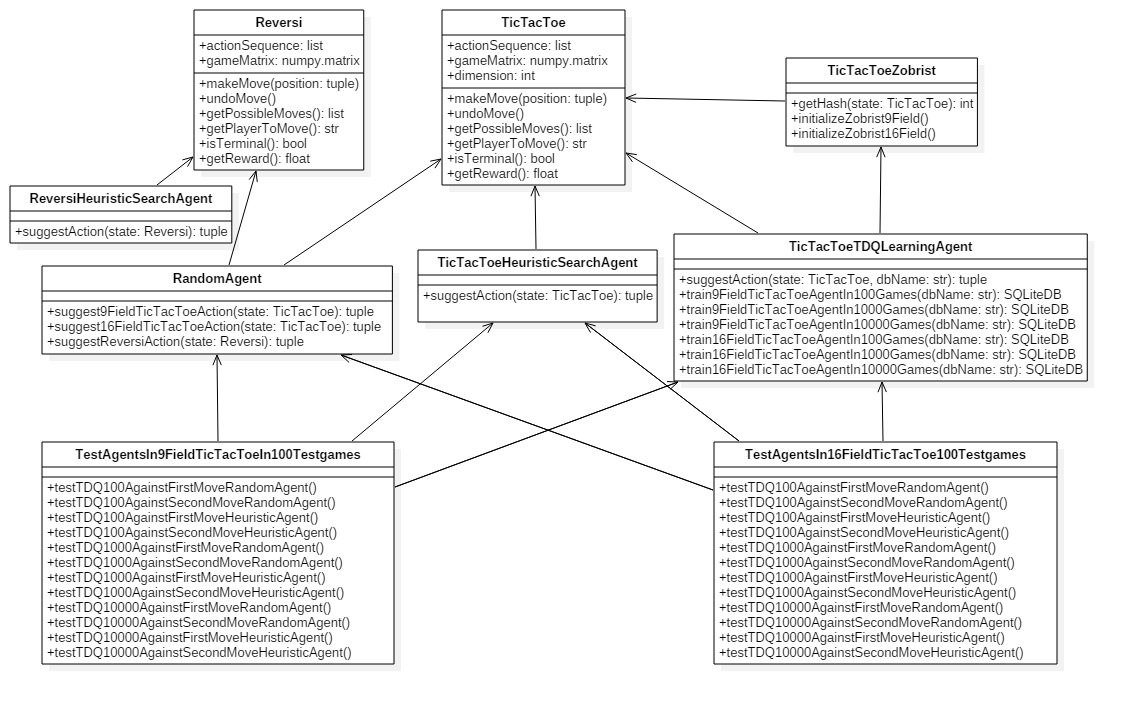
\includegraphics[angle = 90, scale = 0.5]{inhalt/abbildungen/projectClassDiagram.jpg}
  \caption{Klassendiagramm der Software}
  \label{fig:klassendiagramm}
\end{figure} 
